\documentclass[11pt,twocolumn]{article}

\usepackage[hmargin=1.25cm, vmargin=1.5cm]{geometry} % Document margins

\usepackage{amsmath}
\usepackage{amsthm}
\usepackage{graphicx}
\usepackage{mathtools}
\usepackage{fullpage}
\usepackage{verbatim}

\title{Brownian Dynein Model}

\newcommand{\mn}{\scalebox{0.7}[1.0]{-}}

\begin{document}

\maketitle

\section{Both bound}

\begin{figure}
  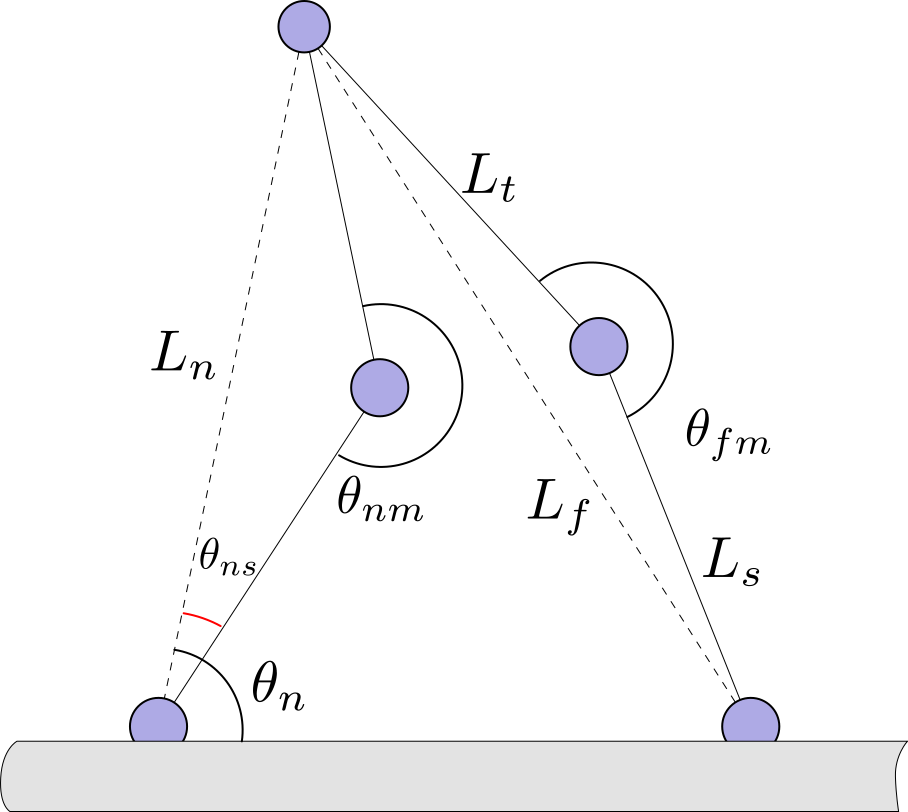
\includegraphics[width=\columnwidth]{../figures/code-bothbound}
  \caption{Angles used in both-bound case.}\label{fig:bothbound}
\end{figure}

In the both-bound case, we use two angles, as illustrated in
Fig.~\ref{fig:bothbound}.

These are the distances to the tail domain from the near and far
binding domains:
\begin{align}
  L_n &= \sqrt{L_s^2 + L_t^2 - 2L_sL_t\cos{\theta_{nm}}} \\
  L_f &= \sqrt{L_s^2 + L_t^2 - 2L_sL_t\cos{\theta_{fm}}}
\end{align}
We use two angles to determine the position of the motor domain:
\begin{align}
  \cos\theta_n &= \frac{L^2 + L_n^2 - L_f^2}{2L L_n} \\
  \sin\theta_{n} &= \sqrt{1 - \cos^2\theta_{n}} \\
  \cos\theta_{ns} &= \frac{L_s^2 + L_n^2 - L_t^2}{2L_s L_n} \\
  \sin\theta_{ns} &=
  \begin{cases}
    +\sqrt{1 - \cos^2\theta_{ns}} & \theta_{nm} < \pi \\
    -\sqrt{1 - \cos^2\theta_{ns}} & \theta_{nm} > \pi
  \end{cases}
\end{align}
Given these definitions, the position of the motor domain is given
simply by $\cos$ and $\sin$ of $\theta_n$ and $\theta_{ns}$:
\begin{align}
  X_{nm} &= L_s\left(
  \cos\theta_n\cos\theta_{ns} - \sin\theta_n\sin\theta_{ns}
  \right)
  \\
  Y_{nm} &= L_s\left(
  \cos\theta_n\sin\theta_{ns} + \sin\theta_n\cos\theta_{ns}
  \right)
\end{align}
Looking at their derivatives gives
\begin{multline}
  \dot{X}_{nm} = L_s\Big(
  \cos\theta_n\dot{\cos\theta_{ns}} + \cos\theta_{ns}\dot{\cos\theta_{n}} \\
  - \sin\theta_n\dot{\sin\theta_{ns}} - \sin\theta_{ns}\dot{\sin\theta_{n}}
  \Big)
\end{multline}
\begin{multline}
  \dot{Y}_{nm} = L_s\Big(
  \cos\theta_n\dot{\sin\theta_{ns}} + \sin\theta_{ns}\dot{\cos\theta_{n}} \\
  + \sin\theta_n\dot{\cos\theta_{ns}} + \cos\theta_{ns}\dot{\sin\theta_{n}}
  \Big)
\end{multline}

C++ code could look like:
\begin{verbatim}
  dXnm_dLn = Ls*(cosAn*dcosAns_dLn
                 + cosAns*dcosAn_dLn
                 - sinAn*dsinAns_dLn
                 - sinAns*dsinAn_dLn);
\end{verbatim}

\section{One bound}

\begin{figure}
  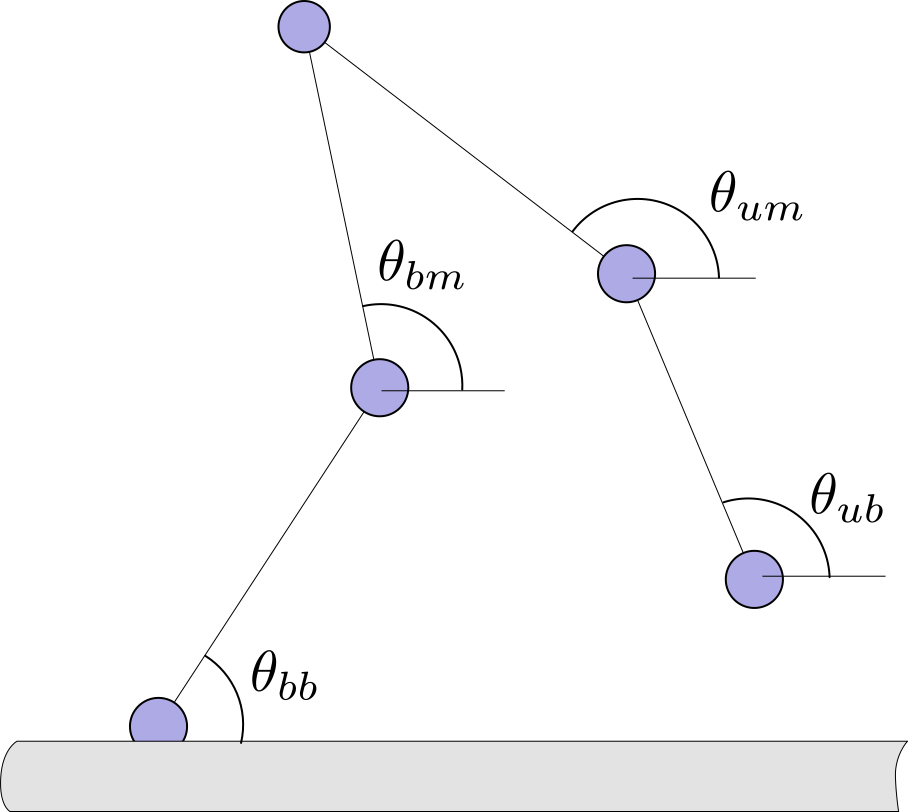
\includegraphics[width=\columnwidth]{../figures/code-onebound}
  \caption{Angles used in one-bound case.}\label{fig:onebound}
\end{figure}

In the one-bound case, we use four angles, as illustrated in
Fig.~\ref{fig:onebound}.

\end{document}
